% ============================================================
% fig_quadrotor_dynamics.tex  — v4, no overlaps
% Requires: \usetikzlibrary{arrows.meta, calc, backgrounds}
% ============================================================
\usetikzlibrary{arrows.meta, calc, backgrounds}

\tikzset{
	vec/.style   ={-{Stealth[length=5pt,width=4pt]}, line width=1.5pt},
	torcarc/.style={-{Stealth[length=4pt,width=3.5pt]}, line width=1.2pt},
}

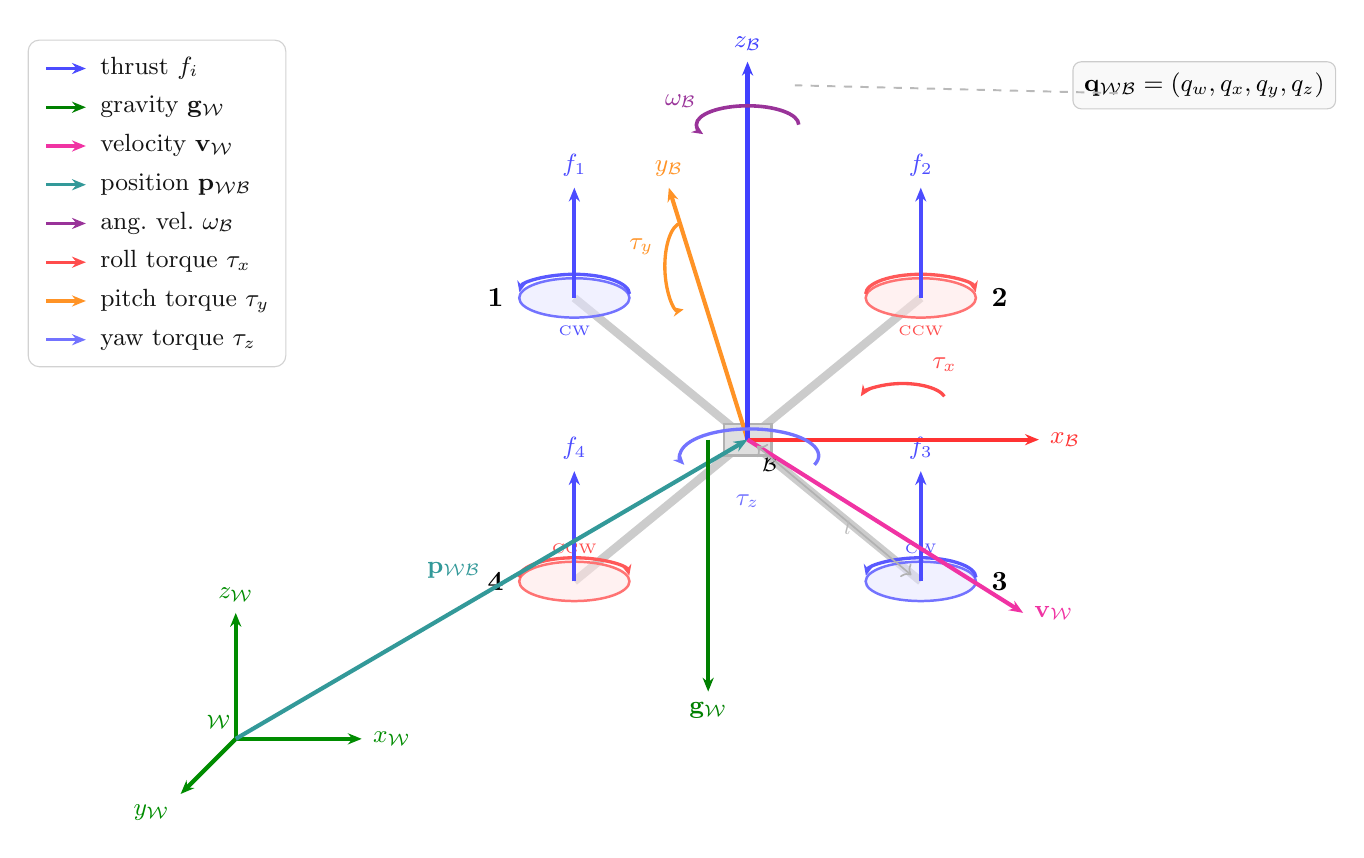
\begin{tikzpicture}[scale=1.0]
	
	% ── centre of mass ──────────────────────────────────────────
	\coordinate (O) at (0,0);
	
	% ── rotor centres  (wide spread, clear separation) ──────────
	%   layout (top view in perspective):
	%     1 = front-left   2 = front-right
	%     4 = back-left    3 = back-right
	\coordinate (A1) at (-2.2,  1.8);
	\coordinate (A2) at ( 2.2,  1.8);
	\coordinate (A3) at ( 2.2, -1.8);
	\coordinate (A4) at (-2.2, -1.8);
	
	% ── arms ────────────────────────────────────────────────────
	\draw[line width=3pt, color=gray!40] (O)--(A1);
	\draw[line width=3pt, color=gray!40] (O)--(A2);
	\draw[line width=3pt, color=gray!40] (O)--(A3);
	\draw[line width=3pt, color=gray!40] (O)--(A4);
	
	% ── body ────────────────────────────────────────────────────
	\filldraw[fill=gray!25, draw=gray!60, line width=1pt]
	(-0.30,-0.20) rectangle (0.30,0.20);
	
	% ── rotor discs  (CW=blue 1,3  CCW=red 2,4) ─────────────────
	\filldraw[fill=blue!10,draw=blue!55,line width=0.9pt,fill opacity=0.55]
	(A1) ellipse (0.70 and 0.25);
	\filldraw[fill=red!10, draw=red!55, line width=0.9pt,fill opacity=0.55]
	(A2) ellipse (0.70 and 0.25);
	\filldraw[fill=blue!10,draw=blue!55,line width=0.9pt,fill opacity=0.55]
	(A3) ellipse (0.70 and 0.25);
	\filldraw[fill=red!10, draw=red!55, line width=0.9pt,fill opacity=0.55]
	(A4) ellipse (0.70 and 0.25);
	
	% ── spin arcs ───────────────────────────────────────────────
	\draw[torcarc,color=blue!65]  % 1 CW
	($(A1)+( 0.70,0.05)$) arc[start angle=0,  end angle=175,
	x radius=0.70, y radius=0.25];
	\draw[torcarc,color=red!65]   % 2 CCW
	($(A2)+(-0.70,0.05)$) arc[start angle=180,end angle=5,
	x radius=0.70, y radius=0.25];
	\draw[torcarc,color=blue!65]  % 3 CW
	($(A3)+( 0.70,0.05)$) arc[start angle=0,  end angle=175,
	x radius=0.70, y radius=0.25];
	\draw[torcarc,color=red!65]   % 4 CCW
	($(A4)+(-0.70,0.05)$) arc[start angle=180,end angle=5,
	x radius=0.70, y radius=0.25];
	
	% ── rotor numbers  (outside the disc, unambiguous side) ─────
	\node[font=\bfseries\normalsize] at ($(A1)+(-1.0, 0.0)$) {1};
	\node[font=\bfseries\normalsize] at ($(A2)+( 1.0, 0.0)$) {2};
	\node[font=\bfseries\normalsize] at ($(A3)+( 1.0, 0.0)$) {3};
	\node[font=\bfseries\normalsize] at ($(A4)+(-1.0, 0.0)$) {4};
	
	% ── CW/CCW labels (below each disc, never touching number) ──
	\node[font=\tiny,color=blue!70] at ($(A1)+(0,-0.42)$) {CW};
	\node[font=\tiny,color=red!70]  at ($(A2)+(0,-0.42)$) {CCW};
	\node[font=\tiny,color=blue!70] at ($(A3)+(0, 0.42)$) {CW};
	\node[font=\tiny,color=red!70]  at ($(A4)+(0, 0.42)$) {CCW};
	
	% ============================================================
	% THRUST FORCES  fi  — straight up, label above disc
	% ============================================================
	\draw[vec,color=blue!70] (A1) -- ++(0,1.4)
	node[above,font=\small,color=blue!70]{$f_1$};
	\draw[vec,color=blue!70] (A2) -- ++(0,1.4)
	node[above,font=\small,color=blue!70]{$f_2$};
	\draw[vec,color=blue!70] (A3) -- ++(0,1.4)
	node[above,font=\small,color=blue!70]{$f_3$};
	\draw[vec,color=blue!70] (A4) -- ++(0,1.4)
	node[above,font=\small,color=blue!70]{$f_4$};
	
	% ============================================================
	% BODY FRAME AXES  — long enough to clear all rotors
	% ============================================================
	% x_B  right
	\draw[vec,color=red!80]    (O) -- ++(3.7, 0.0)
	node[right,font=\small\bfseries,color=red!80]{$x_{\mathcal{B}}$};
	% y_B  upper-left (perspective depth)
	\draw[vec,color=orange!85] (O) -- ++(-1.0, 3.2)
	node[above,font=\small\bfseries,color=orange!85]{$y_{\mathcal{B}}$};
	% z_B  straight up  — well above rotor thrust arrows
	\draw[vec,color=blue!75]   (O) -- ++(0,   4.8)
	node[above,font=\small\bfseries,color=blue!75]{$z_{\mathcal{B}}$};
	
	\node[font=\scriptsize,color=black] at (0.28,-0.32){$\mathcal{B}$};
	
	% ============================================================
	% WORLD FRAME  — far bottom-left, clear of diagram
	% ============================================================
	\coordinate (WO) at (-6.5,-3.8);
	\draw[vec,color=green!55!black] (WO)--++(1.6,0.0)
	node[right,font=\small\bfseries,color=green!55!black]{$x_{\mathcal{W}}$};
	\draw[vec,color=green!55!black] (WO)--++(0,1.6)
	node[above,font=\small\bfseries,color=green!55!black]{$z_{\mathcal{W}}$};
	\draw[vec,color=green!55!black] (WO)--++(-0.7,-0.7)
	node[below left,font=\small\bfseries,color=green!55!black]{$y_{\mathcal{W}}$};
	\node[font=\scriptsize,color=green!55!black]
	at ($(WO)+(-0.22,0.22)$){$\mathcal{W}$};
	
	% ============================================================
	% POSITION  p_{WB}
	% ============================================================
	\draw[vec,color=teal!80,line width=1.5pt] (WO)--(O)
	node[midway,above left,font=\small,color=teal!80]
	{$\mathbf{p}_{\mathcal{WB}}$};
	
	% ============================================================
	% GRAVITY  — offset left of CoM, fully below body
	% ============================================================
	\draw[vec,color=green!50!black]
	(-0.5,0)--(-0.5,-3.2)
	node[below,font=\small,color=green!50!black]{$\mathbf{g}_{\mathcal{W}}$};
	
	% ============================================================
	% LINEAR VELOCITY  — lower-right, away from axes
	% ============================================================
	\draw[vec,color=magenta!80]
	(O)--++(3.5,-2.2)
	node[right,font=\small,color=magenta!80]{$\mathbf{v}_{\mathcal{W}}$};
	
	% ============================================================
	% ANGULAR VELOCITY  omega_B
	% arc placed high on z_B, well above thrust arrows
	% ============================================================
	\draw[torcarc,color=violet!80,line width=1.3pt]
	( 0.65, 4.0) arc[start angle=0, end angle=210,
	x radius=0.65, y radius=0.24];
	\node[font=\small,color=violet!80] at (-0.85, 4.30)
	{$\boldsymbol{\omega}_{\mathcal{B}}$};
	
	% ============================================================
	% ROLL  tau_x
	% arc around x_B axis — placed right side, between O and A2/A3
	% (x_B points right, so arc is in yz-plane at x=2.5)
	% ============================================================
	\draw[torcarc,color=red!70]
	($(O)+(2.5, 0.55)$)
	arc[start angle=15, end angle=165,
	x radius=0.55, y radius=0.22];
	\node[font=\small,color=red!70] at ($(O)+(2.5, 0.95)$)
	{$\tau_x$};
	
	% ============================================================
	% PITCH  tau_y
	% arc around y_B axis — placed on the y_B arm itself (upper-left)
	% at a point midway along y_B, well away from z_B and tau_z
	% ============================================================
	\draw[torcarc,color=orange!85]
	($(O)+(-0.85, 2.75)$)
	arc[start angle=95, end angle=275,
	x radius=0.22, y radius=0.55];
	\node[font=\small,color=orange!85] at ($(O)+(-1.35, 2.45)$)
	{$\tau_y$};
	
	% ============================================================
	% YAW  tau_z
	% arc around z_B axis — placed just above body, below thrust arcs
	% small radius so it does not reach any arm
	% ============================================================
	\draw[torcarc,color=blue!55]
	($(O)+( 0.85,-0.32)$)
	arc[start angle=-20, end angle=200,
	x radius=0.88, y radius=0.34];
	\node[font=\small,color=blue!55] at ($(O)+(0.0,-0.78)$)
	{$\tau_z$};
	
	% ============================================================
	% ATTITUDE  quaternion  — top-right corner, well clear
	% ============================================================
	\node[draw=gray!40,rounded corners=3pt,fill=gray!5,
	font=\small,inner sep=4pt]
	at (5.8, 4.5)
	{$\mathbf{q}_{\mathcal{WB}}=(q_w,q_x,q_y,q_z)$};
	\draw[dashed,line width=0.7pt,color=gray!55]
	(4.7,4.4)--(0.6,4.5);
	
	% ============================================================
	% ARM LENGTH dimension  (between O and A3 arm)
	% ============================================================
	\draw[<->,gray!60,line width=0.6pt]
	(0.12,-0.08) -- ($(A3)+(-0.12,0.08)$)
	node[midway,below right,font=\scriptsize,color=gray!55]{$l$};
	
	% ============================================================
	% LEGEND  — far top-left, clear of everything
	% ============================================================
	\begin{scope}[on background layer]
		\node[draw=gray!35,fill=white,fill opacity=0.92,
		rounded corners=4pt,inner sep=6pt,
		align=left,font=\small]
		at (-7.5, 3.0) {%
			\tikz\draw[vec,color=blue!70,line width=1.2pt](0,0)--(0.5,0);%
			\enspace thrust $f_i$\\[3pt]
			\tikz\draw[vec,color=green!50!black,line width=1.2pt](0,0)--(0.5,0);%
			\enspace gravity $\mathbf{g}_{\mathcal{W}}$\\[3pt]
			\tikz\draw[vec,color=magenta!80,line width=1.2pt](0,0)--(0.5,0);%
			\enspace velocity $\mathbf{v}_{\mathcal{W}}$\\[3pt]
			\tikz\draw[vec,color=teal!80,line width=1.2pt](0,0)--(0.5,0);%
			\enspace position $\mathbf{p}_{\mathcal{WB}}$\\[3pt]
			\tikz\draw[vec,color=violet!80,line width=1.2pt](0,0)--(0.5,0);%
			\enspace ang.\ vel.\ $\boldsymbol{\omega}_{\mathcal{B}}$\\[3pt]
			\tikz\draw[vec,color=red!70,line width=1.2pt](0,0)--(0.5,0);%
			\enspace roll torque $\tau_x$\\[3pt]
			\tikz\draw[vec,color=orange!85,line width=1.2pt](0,0)--(0.5,0);%
			\enspace pitch torque $\tau_y$\\[3pt]
			\tikz\draw[vec,color=blue!55,line width=1.2pt](0,0)--(0.5,0);%
			\enspace yaw torque $\tau_z$
		};
	\end{scope}
	
\end{tikzpicture}